\documentclass[10pt,a4paper]{amsart}
\usepackage{amsmath,amssymb,amsthm,graphicx}
\usepackage{amsmath,amssymb,graphicx,xcolor,mathtools}
\title{Transfer of coherence along Tietze equivalences of underlying0-polygraphs}
\author{Samuel Mimram, Émile Oleon}
\date{doi:10.4230/LIPIcs.FSCD.2025.30; CC BY4.0 (official paper and diagrams)}
\begin{document}
\maketitle
\noindent\textit{Editorial note.} Source https://drops.dagstuhl.de/entities/document/10.4230/LIPIcs.FSCD.2025.30. © Samuel Mimram and Émile Oleon, CC BY4.0. Complete author natural-language proof and original diagrams retained.\par\medskip
\noindent\textit{Editorial note.} The transfer theorem retains the author coherence hypothesis and complete constructive proof. The separate choice-dependent completeness theorem is not used as a new assumption.\par\medskip
\noindent\textit{Allowed standard prerequisites (editorial).}\begin{itemize}
\item Homotopy type theory, higher inductive realizations, paths/cells and elementary Tietze transformations. Complete author §§1–2.2 and §3 definitions/proofs retained. The axiom of choice used in the separate completeness section is not introduced as an assumption for this transfer theorem.
\end{itemize}\medskip
% BEGIN S1
 
\par\medskip\noindent\textbf{1 1-polygraphs}\par
 
% BEGIN S1.p1
 
Before introducing 1-polygraphs, we first need to present the (quite trivial) 0-dimensional variant. A 0-polygraph $P$ is simply a type whose elements are called $0$-generators. A sphere $(x,y)$ in a 0-polygraph $P$ is a pair of elements of $P$, and we write $\operatorname{S}P$ for the type of such objects. If we write $\operatorname{S}^{0}=\{0,1\}$ for the type with two elements, corresponding to the canonical 0-sphere, it can be noted that a sphere in a 0-polygraph $P$ corresponds to an arrow $\operatorname{S}^{0}\to P$. Given a $0$-polygraph $P$, we call $\|P\|_{-1}$ the proposition presented by $P$.\par
 
% END S1.p1
 
% BEGIN S1.SS1
 
\par\medskip\noindent\textbf{1.1 Internal and external 1-polygraphs}\par
 
% BEGIN S1.SS1.SSS0.P0.SPx1
 
\par\medskip\noindent\textbf{1-polygraphs.}\par
 
% BEGIN S1.SS1.SSS0.P0.SPx1.p1
 
A 1-polygraph $P$ consists of a 0-polygraph $\operatorname{U}P$ (the underlying 0-polygraph of $P$) together with a function $\operatorname{S}{\operatorname{U}P}\to\mathcal{U}$, which to any sphere $(x,y)$ in the underlying 0-polygraph associates a type $P(x,y)$ whose elements are called the 1-generators of the 1-polygraph. In other words, 1-polygraphs correspond to type-theoretic directed graphs. A 1-polygraph is discrete when all the types $\operatorname{U}P$ and $P(x,y)$ are sets. In the following, a sphere in $\operatorname{U}P$ is called a 0-sphere of $P$.\par
 
% END S1.SS1.SSS0.P0.SPx1.p1
 
% END S1.SS1.SSS0.P0.SPx1
 
% BEGIN S1.SS1.SSS0.P0.SPx2
 
\par\medskip\noindent\textbf{1-generators.}\par
 
% BEGIN S1.SS1.SSS0.P0.SPx2.p1
 
The elements of $\operatorname{U}P$ are called 0-generators or 0-cells of $P$. We sometimes write $\operatorname{S}_{0}P:=\operatorname{S}\operatorname{U}P$ for the 0-spheres, as well as $P_{0}:=\operatorname{U}P$ and $P_{1}:=\Sigma((x,y):\operatorname{S}_{0}P).P(x,y)$ for the type of 0- and 1-generators of $P$. We also write $\partial^{-},\partial^{+}:P_{1}\to P_{0}$ for the source and target functions (defined by $\partial^{-}:=\pi\circ\pi$ and $\partial^{+}:=\pi^{\prime}\circ\pi$).\par
 
% END S1.SS1.SSS0.P0.SPx2.p1
 
% END S1.SS1.SSS0.P0.SPx2
 
% BEGIN S1.SS1.SSS0.P0.SPx3
 
\par\medskip\noindent\textbf{1-cells.}\par
 
% BEGIN S1.SS1.SSS0.P0.SPx3.p1
 
Given a 1-polygraph $P$ and a $0$-sphere $(x,y)$, we write $P^{*}(x,y)$ for the type of 1-cells in $P$ from $x$ to $y$. This family of types is defined inductively as the smallest one such that\par
  
\par\noindent  $\blacksquare$ 
% BEGIN S1.I1.i1.p1
 
for every 0-cell $x:\operatorname{U}P$, we have a 1-cell $\operatorname{id}_{x}:P^{*}(x,x)$,\par
 
% END S1.I1.i1.p1
 
 
\par\noindent  $\blacksquare$ 
% BEGIN S1.I1.i2.p1
 
for every 0-cells $x,y,z:\operatorname{U}P$, 1-generator $a:P(x,y)$ and $1$-cell $u:P^{*}(y,z)$, we have a 1-cell $a::u:P^{*}(x,z)$,\par
 
% END S1.I1.i2.p1
 
 
\par\noindent  $\blacksquare$ 
% BEGIN S1.I1.i3.p1
 
for every 0-cells $x,y,z:\operatorname{U}P$, 1-generator $a:P(y,x)$ and $1$-cell $u:P^{*}(y,z)$, we have a 1-cell $a::^{\prime}u:P^{*}(x,z)$.\par
 
% END S1.I1.i3.p1
 
  
Informally, cells in $P^{*}(x,y)$ are undirected paths from $x$ to $y$ in the graph corresponding to $P$ (where the two last cases respectively correspond to taking an arrow $a$ forward and backward). In the following, we often write $a:x\to y$ for a 1-generator $a:P(x,y)$ and $u:x\overset{*}{\to}y$ for a 1-cell $u:P^{*}(x,y)$.\par
 
% END S1.SS1.SSS0.P0.SPx3.p1
 
% END S1.SS1.SSS0.P0.SPx3
 
% BEGIN S1.SS1.SSS0.P0.SPx4
 
\par\medskip\noindent\textbf{Composition.}\par
 
% BEGIN S1.SS1.SSS0.P0.SPx4.p1
 
Given two 1-cells $u:x\overset{*}{\to}y$ and $v:y\overset{*}{\to}z$, we define their composite $u\cdot{}v:x\overset{*}{\to}z$ by induction on $u$ by\par
    $\displaystyle\operatorname{id}\cdot{}v$ $\displaystyle:=v$ $\displaystyle(a::u)\cdot{}v$ $\displaystyle:=a::(u\cdot{}v)$ $\displaystyle(a::^{\prime}u)\cdot{}v$ $\displaystyle:=a::^{\prime}(u\cdot{}v)$    
% END S1.SS1.SSS0.P0.SPx4.p1
 
% BEGIN Thmtheorem1
 
\par\medskip\noindent\textbf{Lemma 1 ([13, comp0-assoc]).}\par
 
% BEGIN Thmtheorem1.p1
 
Composition is associative and unital.\par
 
% END Thmtheorem1.p1
 
% END Thmtheorem1
 
% BEGIN S1.SS1.SSS0.P0.SPx4.p2
 
Given a 1-cell $u:x\overset{*}{\to}y$, we define its opposite $u^{\mathrm{op}}:y\overset{*}{\to}x$ by induction on $u$ by\par
    $\displaystyle\operatorname{id}^{\mathrm{op}}$ $\displaystyle:=\operatorname{id}$ $\displaystyle(a::u)^{\mathrm{op}}$ $\displaystyle:=a\mathbin{\overline{::}^{\prime}}u^{\mathrm{op}}$ $\displaystyle(a::^{\prime}u)^{\mathrm{op}}$ $\displaystyle:=a\mathbin{\overline{::}}u^{\mathrm{op}}$    
where $a\mathbin{\overline{::}}u$, which corresponds to appending $a$ to $u$, is defined by\par
    $\displaystyle a\mathbin{\overline{::}}\operatorname{id}$ $\displaystyle:=a::\operatorname{id}$ $\displaystyle a\mathbin{\overline{::}}(b::u)$ $\displaystyle:=b::(a\mathbin{\overline{::}}u)$ $\displaystyle a\mathbin{\overline{::}}(b::^{\prime}u)$ $\displaystyle:=b::^{\prime}(a\mathbin{\overline{::}}u)$    
and $a\mathbin{\overline{::}^{\prime}}u$, corresponding to appending $a$ backward to $u$, is defined similarly.\par
 
% END S1.SS1.SSS0.P0.SPx4.p2
 
% END S1.SS1.SSS0.P0.SPx4
 
% BEGIN S1.SS1.SSS0.P0.SPx5
 
\par\medskip\noindent\textbf{Spheres.}\par
 
% BEGIN S1.SS1.SSS0.P0.SPx5.p1
 
A sphere $s$ in a 1-polygraph $P$ consists of a $0$-sphere $(x,y)$ together with a pair of 1-cells $f,g:x\overset{*}{\to}y$. The underlying 0-sphere $(x,y)$ is noted $\operatorname{U}s$. The cell $f$ (resp. $g$) is called the source (resp. target) of $s$ and noted $\partial^{-}s$ (resp. $\partial^{+}s$), so that the sphere $s$ is the triple $(\operatorname{U}s,\partial^{-}s,\partial^{+}s)$. We write $\operatorname{S}P$ for type of spheres in a $1$-polygraph.\par
 
% END S1.SS1.SSS0.P0.SPx5.p1
 
% END S1.SS1.SSS0.P0.SPx5
 
% BEGIN S1.SS1.SSS0.P0.SPx6
 
\par\medskip\noindent\textbf{Coherent 1-cells.}\par
 
% BEGIN S1.SS1.SSS0.P0.SPx6.p1
 
In the definition of 1-cell, we think of $a::-$ and $a::^{\prime}-$ as respectively precomposing by the 1-cell $a$ and its inverse. However, nothing enforces that they are actually inverse operations, i.e. that we have\par
    $\displaystyle a::^{\prime}a::u$ $\displaystyle=u$ $\displaystyle a::a::^{\prime}u$ $\displaystyle=u$    
for any 1-generator $a$ and 1-cell $u$ of suitable types. We define the types of coherent 1-cells $P^{\sim}(x,y)$, indexed by 0-spheres $(x,y)$, as the quotient of the types of 1-cells $P^{*}(x,y)$ under the congruence generated by the above relations. This type is the “right” definition for the 1-cells of $P$, in the sense that it gives a description of the free groupoid generated by $P$ [9]. However, non coherent 1-cells provides representatives for those which are often simpler to work with. Namely, by definition of coherent 1-cells as a quotient of 1-cells, we have\par
 
% END S1.SS1.SSS0.P0.SPx6.p1
 
% BEGIN Thmtheorem2
 
\par\medskip\noindent\textbf{Lemma 2.}\par
 
% BEGIN Thmtheorem2.p1
 
For $x,y:\operatorname{U}P$, the canonical map $f:P^{*}(x,y)\to P^{\sim}(x,y)$ is a surjection, i.e. the type $\|\operatorname{hfib}_{f}(u)\|_{-1}$ is inhabited for any $u:P^{\sim}(x,y)$.\par
 
% END Thmtheorem2.p1
 
% END Thmtheorem2
 
% END S1.SS1.SSS0.P0.SPx6
 
% END S1.SS1
 
% BEGIN S1.SS2
 
\par\medskip\noindent\textbf{1.2 Geometric realization}\par
 
% BEGIN S1.SS2.p1
 
We introduce the “geometric realization” of a 1-polygraph $P$, which can be thought of as a type-theoretical graph with $P_{0}$ as vertices and $P_{1}$ as edges. The set presented by $P$ is then defined as the type of connected components of this graph.\par
 
% END S1.SS2.p1
 
% BEGIN S1.SS2.SSS0.P0.SPx1
 
\par\medskip\noindent\textbf{Geometric realization.}\par
 
% BEGIN S1.SS2.SSS0.P0.SPx1.p1
 
Given a 1-polygraph $P$ its geometric realization $\overline{P}$ is the higher inductive type generated by the two constructors\par
    $\displaystyle\iota:\operatorname{U}P$ $\displaystyle\to\overline{P}$ $\displaystyle\gamma:((x,y):\operatorname{S}_{0}P)\to P(x,y)$ $\displaystyle\to\iota x=\iota y$    
More abstractly, it corresponds to the pushout on the left or to the coequalizer on the right\par
    
\begin{center}
\includegraphics[width=0.95\linewidth,height=0.42\textheight,keepaspectratio]{graph-01.pdf}\end{center}
    
where the horizontal arrow $f$ sends an edge $a:x\to y$ and $0$ (resp. $1$) to $x$ (resp. $y$), which corresponds to attaching 1-cells to a 0-dimensional cell complex. The associated induction principle is the following.\par
 
% END S1.SS2.SSS0.P0.SPx1.p1
 
% BEGIN Thmtheorem3
 
\par\medskip\noindent\textbf{Proposition 3.}\par
 
% BEGIN Thmtheorem3.p1
 
Suppose given an arbitrary type $A$. Any two functions $f_{0}:P_{0}\to A$ and $f_{1}:(((x,y),a):P_{1})\to f_{0}(x)=f_{0}(y)$ induce a unique function $f:\overline{P}\to A$ such that $f\circ\iota=f_{0}$ and $f\circ\gamma=f_{1}$. We also have the expected dependent generalization.\par
 
% END Thmtheorem3.p1
 
% END Thmtheorem3
 
% BEGIN S1.SS2.SSS0.P0.SPx1.p2
 
By partial evaluation, the map $\gamma$ induces, for $(x,y):\operatorname{S}_{0}P$, a map $\gamma_{x,y}:P(x,y)\to\iota x=\iota y$, which extends as a map on cells $\gamma^{*}_{x,y}:P^{*}(x,y)\to\iota x=\iota y$ defined by induction by\par
    $\displaystyle\gamma^{*}_{x,x}(\operatorname{id})$ $\displaystyle:=\operatorname{refl}$ $\displaystyle\gamma^{*}_{z,y}(a::u)$ $\displaystyle:=\gamma a\cdot{\gamma^{*}_{x,y}(u)}$ $\displaystyle\gamma^{*}_{z,y}(a::^{\prime}u)$ $\displaystyle:=\gamma a^{-}\cdot{\gamma^{*}_{x,y}(u)}$    
Moreover, since this definition is compatible with the relations for coherent 1-cells, for every sphere $(x,y):\operatorname{S}_{0}P$ we have the following.\par
 
% END S1.SS2.SSS0.P0.SPx1.p2
 
% BEGIN Thmtheorem4
 
\par\medskip\noindent\textbf{Lemma 4.}\par
 
% BEGIN Thmtheorem4.p1
 
The map $\gamma^{*}_{x,y}$ induces a map $\gamma^{\sim}_{x,y}:P^{\sim}(x,y)\to\iota x=\iota y$.\par
 
% END Thmtheorem4.p1
 
% END Thmtheorem4
 
% BEGIN S1.SS2.SSS0.P0.SPx1.p3
 
This map is an equivalence, so it provides a characterization of the paths in geometric realizations of graphs [13, KvR/1Polygraph/PathPresentation.agda]:\par
 
% END S1.SS2.SSS0.P0.SPx1.p3
 
% BEGIN Thmtheorem5
 
\par\medskip\noindent\textbf{Theorem 5.}\par
 
% BEGIN Thmtheorem5.p1
 
The map $\gamma^{\sim}_{x,y}:P^{\sim}(x,y)\to\iota x=\iota y$ is an equivalence.\par
 
% END Thmtheorem5.p1
 
% END Thmtheorem5
 
% END S1.SS2.SSS0.P0.SPx1
 
% BEGIN S1.SS2.SSS0.P0.SPx2
 
\par\medskip\noindent\textbf{Proof.}\par
 
% BEGIN S1.SS2.SSS0.P0.SPx2.p1
 
A map $\iota x=\iota y\to P^{\sim}(x,y)$ can be defined using the elimination principle for paths in $\overline{P}$ given in [9, Theorem 3], and both can be shown to be mutually inverse by induction. $\hfill\blacktriangleleft$\par
 
% END S1.SS2.SSS0.P0.SPx2.p1
 
% END S1.SS2.SSS0.P0.SPx2
 
% BEGIN S1.SS2.SSS0.P0.SPx3
 
\par\medskip\noindent\textbf{Presented set.}\par
 
% BEGIN S1.SS2.SSS0.P0.SPx3.p1
 
The set presented by a 1-polygraph $P$ is the set of connected components of its geometric realization $\|\overline{P}\|_{0}$. This notion is to be understood as an analogue of a group presentation with generators and relations, but shifted down by one dimension: here, the 0-cells of $P$ are the generators of the presented set, and the 1-cells are the relations.\par
 
% END S1.SS2.SSS0.P0.SPx3.p1
 
% BEGIN Thmtheorem6
 
\par\medskip\noindent\textbf{Example 6.}\par
 
% BEGIN Thmtheorem6.p1
 
Consider the polygraph $P$ with $\operatorname{U}P=\mathbb{Z}$ and one relation $a_{n}:n\to n+2$ for $n\in\mathbb{Z}$. The presented set is $\mathbb{Z}_{2}$.\par
 
% END Thmtheorem6.p1
 
% END Thmtheorem6
 
% BEGIN S1.SS2.SSS0.P0.SPx3.p2
 
We now prove some technical lemmas that will be useful later on.\par
 
% END S1.SS2.SSS0.P0.SPx3.p2
 
% BEGIN Thmtheorem7
 
\par\medskip\noindent\textbf{Lemma 7.}\par
 
% BEGIN Thmtheorem7.p1
 
For $x,y:\operatorname{U}P$ and $p:|\iota(x)|_{0}=|\iota(y)|_{0}$ in $\|\overline{P}\|_{0}$, there merely exists a 1-cell $x\overset{*}{\to}y$ in $P$.\par
 
% END Thmtheorem7.p1
 
% END Thmtheorem7
 
% END S1.SS2.SSS0.P0.SPx3
 
% BEGIN S1.SS2.SSS0.P0.SPx4
 
\par\medskip\noindent\textbf{Proof.}\par
 
% BEGIN S1.SS2.SSS0.P0.SPx4.p1
 
By [19, Theorem 7.3.12], the type $|\iota(x)|_{0}=|\iota(y)|_{0}$ coincides with $\|\iota(x)=\iota(y)\|_{-1}$. Since we are eliminating to a proposition, we can suppose given a path $p:\iota(x)=\iota(y)$ which by Theorem 5 induces a coherent cell $\tilde{p}:P^{\sim}(x,y)$, and we conclude by Lemma 2. $\hfill\blacktriangleleft$ The following shows that we can pick a representative 0-cell in every connected component [13, has-repr]:\par
 
% END S1.SS2.SSS0.P0.SPx4.p1
 
% BEGIN Thmtheorem8
 
\par\medskip\noindent\textbf{Proposition 8.}\par
 
% BEGIN Thmtheorem8.p1
 
The type $\Pi(x:\|\overline{P}\|_{0}).\|\Sigma(\hat{x}:\operatorname{U}P).|\iota(\hat{x})|_{0}=x\|_{-1}$ is inhabited.\par
 
% END Thmtheorem8.p1
 
% END Thmtheorem8
 
% END S1.SS2.SSS0.P0.SPx4
 
% BEGIN S1.SS2.SSS0.P0.SPx5
 
\par\medskip\noindent\textbf{Proof.}\par
 
% BEGIN S1.SS2.SSS0.P0.SPx5.p1
 
Any proposition being a set [19, Lemma 3.3.4], it is enough to construct a map $f:\Pi(x:\overline{P}).\|\Sigma(\hat{x}:\operatorname{U}P).\iota(\hat{x})=x\|_{-1}$ which can be done by using the elimination principle of $\overline{P}$ (Proposition 3). Namely, we define, for $x:\operatorname{U}P$, $f(\iota(x)):=|(x,\operatorname{refl}_{\iota(x)})|_{-1}$ and, for $x,y:\operatorname{U}P$ and $a:P(x,y)$, the path associated to it by $f$ is canonically defined by the fact that we are eliminating to a proposition. $\hfill\blacktriangleleft$\par
 
% END S1.SS2.SSS0.P0.SPx5.p1
 
% END S1.SS2.SSS0.P0.SPx5
 
% END S1.SS2
 
% END S1


% BEGIN S2
 
\par\medskip\noindent\textbf{2 Tietze transformations}\par
 
% BEGIN S2.p1
 
Tietze transformations originate from the work of Tietze [18] who defined two transformations on group presentations:\par
  (T0)  
% BEGIN S2.I1.ix1.p1
 
adding a definable generator,\par
 
% END S2.I1.ix1.p1
  (T1)  
% BEGIN S2.I1.ix2.p1
 
adding a derivable relation.\par
 
% END S2.I1.ix2.p1
   
The equivalence relation they induce, the Tietze equivalence, characterizes when two presentations give rise to the same group, up to isomorphism. These transformations have then been generalized to a variety of contexts, including the very general one of polygraphs [1, 5] for presentations of (higher) categories, and have as well been shown to provide a interesting notion of weak equivalence [7]. Their fundamental property can be decomposed in two parts:\par
  
\par\noindent  $\blacksquare$ 
% BEGIN S2.I2.i1.p1
 
correctness: any two presentations which are Tietze equivalent present the same structure,\par
 
% END S2.I2.i1.p1
 
 
\par\noindent  $\blacksquare$ 
% BEGIN S2.I2.i2.p1
 
completeness: any two presentations of the same structure are Tietze equivalent.\par
 
% END S2.I2.i2.p1
 
  
Here, we think of a 1-polygraph $P$ as presenting the set $\|\overline{P}\|_{0}$, and we define elementary transformations as explained above. We then show that they are correct and complete with respect to the presented set.\par
 
% END S2.p1
 
% BEGIN S2.SS1
 
\par\medskip\noindent\textbf{2.1 Definition}\par
 
% BEGIN S2.SS1.p1
 
We define the two following families of Tietze transformations, which transform a given 1-polygraph $P$ into another 1-polygraph, by attaching cells to it:\par
  (T0)  
% BEGIN S2.I3.ix1.p1
 
Add a definable 0-generator: given a type $X$ and a function $\partial:X\to\operatorname{U}P$, we construct the polygraph $P{\uparrow_{0}}\partial$ defined, for $(x,y):\operatorname{S}_{0}P$, by\par
    $\displaystyle\operatorname{U}(P{\uparrow_{0}}\partial)$ $\displaystyle:=\operatorname{U}P\sqcup X$ $\displaystyle(P{\uparrow_{0}}\partial)(x,y)$ $\displaystyle:=\begin{cases}P(x,y)&\text{if $x:\operatorname{U}P$ and $y:\operatorname{U}P$}\\
x=\partial(y)&\text{if $x:\operatorname{U}P$ and $y:X$}\\
\bot&\text{otherwise}\end{cases}$    
% END S2.I3.ix1.p1
  (T1)  
% BEGIN S2.I3.ix2.p1
 
Add a derivable relation: given a function $\partial:\operatorname{S}_{0}P\to\mathcal{U}$ and a family of functions $\partial_{x,y}:\partial(x,y)\to(x\overset{*}{\to}y)$ indexed by 0-spheres $(x,y):\operatorname{S}_{0}P$, we construct the polygraph $P{\uparrow_{1}}\partial$ defined, for $(x,y):\operatorname{S}_{0}P$, by\par
    $\displaystyle\operatorname{U}(P{\uparrow_{1}}\partial)$ $\displaystyle:=\operatorname{U}P$ $\displaystyle(P{\uparrow_{1}}\partial)(x,y)$ $\displaystyle:=P(x,y)\sqcup\partial(x,y)$    
% END S2.I3.ix2.p1
   
A transformation (T0) consists in adding, for every element $x:X$, a new 0-generator $x$ to the polygraph together with a 1-generator $\tau_{x}:\partial x\to x$:\par
    
\begin{center}
\includegraphics[width=0.95\linewidth,height=0.42\textheight,keepaspectratio]{graph-02.pdf}\end{center}
    
with $y\overset{\text{def}}{=}\partial x$, and $\tau_{x}$ is a notation for the element $\operatorname{refl}_{x}:(P{\uparrow_{0}}\partial)(y,x)$. A transformation (T1) consists in adding, for every $x,y:X$ and $a:\partial(x,y)$, a 1-generator $a:x\to y$:\par
    
\begin{center}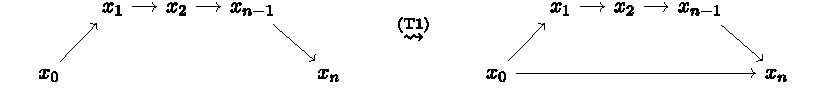
\includegraphics[width=0.95\linewidth,height=0.42\textheight,keepaspectratio]{graph-03.pdf}\end{center}
    
It can be observed that we have a new hole after performing a transformation (T1), which justifies the importance of the set-truncation in the definition of the presented set. Note that the functions $\partial_{x,y}$ are not used in order to define $Q$ in (T1), but they will be necessary to show the correctness of the transformation below. For instance, if we did not require those, we could make any polygraph coherent by taking $\partial(x,y)=\top$ for any $(x,y):\operatorname{S}_{0}P$.\par
 
% END S2.SS1.p1
 
% BEGIN Thmtheorem9
 
\par\medskip\noindent\textbf{$\blacktriangleright$ Remark 9.}\par
 
% BEGIN Thmtheorem9.p1
 
We could also consider a weaker notion of transformation (T1) where we only require the existence of the 1-cell associated to an added 1-generator, i.e. type the function as $\partial_{x,y}:\partial(x,y)\to\|x\overset{*}{\to}y\|_{-1}$. This variant would in fact be enough for the subsequent developments here.\par
 
% END Thmtheorem9.p1
 
% END Thmtheorem9
 
% BEGIN Thmtheorem10
 
\par\medskip\noindent\textbf{Example 10.}\par
 
% BEGIN Thmtheorem10.p1
 
We have the following series of Tietze transformations:\par
    
\begin{center}
\includegraphics[width=0.95\linewidth,height=0.42\textheight,keepaspectratio]{graph-04.pdf}\end{center}
    
% END Thmtheorem10.p1
 
% END Thmtheorem10
 
% BEGIN S2.SS1.p2
 
Under the Grothendieck duality between type families and fibrations [19, Section 4.8], the Tietze transformations (T1) can reformulated as follows (a similar reformulation for (T0) could also be given):\par
 
% END S2.SS1.p2
 
% BEGIN Thmtheorem11
 
\par\medskip\noindent\textbf{Proposition 11.}\par
 
% BEGIN Thmtheorem11.p1
 
Transformations (T1) are equivalent to the following:\par
  (T1’)  
% BEGIN S2.I4.ix1.p1
 
Given a type $X:\mathcal{U}$ and function $\partial:X\to\Sigma((x,y):\operatorname{S}_{0}P).P^{*}(x,y)$, we construct the polygraph $P{\uparrow_{1}}\partial$ with $\operatorname{U}(P{\uparrow_{1}}\partial):=\operatorname{U}P$ and, for $(x,y):\operatorname{S}P$,\par
    \[(P{\uparrow_{1}}\partial)(x,y):=P(x,y)\sqcup\operatorname{hfib}_{\pi\circ\partial}(x,y)\]    
% END S2.I4.ix1.p1
   
% END Thmtheorem11.p1
 
% END Thmtheorem11
 
% BEGIN S2.SS1.p3
 
We define the Tietze equivalence as the equivalence relation generated by (T0) and (T1).\par
 
% END S2.SS1.p3
 
% BEGIN S2.SS1.SSS0.P0.SPx1
 
\par\medskip\noindent\textbf{Transformations for 0-polygraphs.}\par
 
% BEGIN S2.SS1.SSS0.P0.SPx1.p1
 
The notion of Tietze transformation generalizes to polygraphs in any dimension. In particular, for 0-polygraphs, it can be formulated as follows. An elementary Tietze transformation of 0-polygraphs consists in\par
  (T0)  
% BEGIN S2.I5.ix1.p1
 
Given a 0-polygraph $P$, a type $X$ and a function $\partial:X\to P$, we consider the 0-polygraph $P{\uparrow_{0}}\partial:=P\sqcup X$.\par
 
% END S2.I5.ix1.p1
   
Two 0-polygraphs are Tietze equivalent when they are related by the smallest equivalence relation identifying $P$ with $P{\uparrow_{0}}\partial$ for any $P$ and $\partial$.\par
 
% END S2.SS1.SSS0.P0.SPx1.p1
 
% BEGIN Thmtheorem12
 
\par\medskip\noindent\textbf{Proposition 12.}\par
 
% BEGIN Thmtheorem12.p1
 
There exists a Tietze equivalence between two 0-polygraphs $P$ and $Q$ if and only if they present the same proposition, i.e. $\|P\|_{-1}=\|Q\|_{-1}$.\par
 
% END Thmtheorem12.p1
 
% END Thmtheorem12
 
% END S2.SS1.SSS0.P0.SPx1
 
% END S2.SS1
 
% BEGIN S2.SS2
 
\par\medskip\noindent\textbf{2.2 Correctness}\par
 
% BEGIN S2.SS2.p1
 
Our aim is now to show the correctness property for Tietze transformations of 1-polygraphs: equivalent 1-polygraphs present the same set.\par
 
% END S2.SS2.p1
 
% BEGIN Thmtheorem13
 
\par\medskip\noindent\textbf{Theorem 13 (Correctness).}\par
 
% BEGIN Thmtheorem13.p1
 
Given two Tietze equivalent 1-polygraphs $P$ and $Q$, we have $\|\overline{P}\|_{0}=\|\overline{Q}\|_{0}$.\par
 
% END Thmtheorem13.p1
 
% END Thmtheorem13
 
% BEGIN S2.SS2.p2
 
By induction on the equivalence, it is enough to show the result when $Q$ is obtained form $P$ by a Tietze transformation (T0) or (T1), which we do below. Throughout the section, we suppose fixed a 1-polygraph $P$. We first show that transformations (T0) are correct [13, tietze0-correct]:\par
 
% END S2.SS2.p2
 
% BEGIN Thmtheorem14
 
\par\medskip\noindent\textbf{Proposition 14.}\par
 
% BEGIN Thmtheorem14.p1
 
Given a type $X$ and a function $\partial:X\to\operatorname{U}P$, we have $\|\overline{P}\|_{0}=\|\overline{P{\uparrow_{0}}\partial}\|_{0}$.\par
 
% END Thmtheorem14.p1
 
% END Thmtheorem14
 
% BEGIN S2.SS2.SSS0.P0.SPx1
 
\par\medskip\noindent\textbf{Proof.}\par
 
% BEGIN S2.SS2.SSS0.P0.SPx1.p1
 
By definition of $P{\uparrow_{0}}\partial$ and its geometric realization, we have a coequalizer\par
    
\begin{center}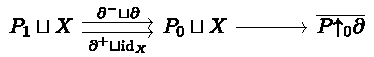
\includegraphics[width=0.95\linewidth,height=0.42\textheight,keepaspectratio]{graph-05.pdf}\end{center}
    
By computing the coequalizer partially on the left component of the coproduct, we find that $\overline{P{\uparrow_{0}}\partial}$ is the coequalizer of $\begin{matrix}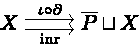
\includegraphics[width=0.24\linewidth,height=0.12\textheight,keepaspectratio]{graph-06.pdf}\end{matrix}$. From which we easily deduce $\overline{P{\uparrow_{0}}\partial}=\overline{P}$. $\hfill\blacktriangleleft$ The transformations (T0) actually preserve, not only the presented set, but also the geometric realization. We now show that transformations (T1) are correct [13, tietze1-correct]:\par
 
% END S2.SS2.SSS0.P0.SPx1.p1
 
% BEGIN Thmtheorem15
 
\par\medskip\noindent\textbf{Proposition 15.}\par
 
% BEGIN Thmtheorem15.p1
 
Given a type $X$, a function $\partial:\operatorname{S}_{0}P\to\mathcal{U}$, and a family of functions $\partial_{x,y}:\partial(x,y)\to(x\overset{*}{\to}y)$ indexed by 0-spheres $(x,y):\operatorname{S}_{0}P$, we have $\|\overline{P}\|_{0}=\|\overline{P{\uparrow_{1}}\partial}\|_{0}$.\par
 
% END Thmtheorem15.p1
 
% END Thmtheorem15
 
% END S2.SS2.SSS0.P0.SPx1
 
% BEGIN S2.SS2.SSS0.P0.SPx2
 
\par\medskip\noindent\textbf{Proof.}\par
 
% BEGIN S2.SS2.SSS0.P0.SPx2.p1
 
By using the induction principle of geometric realization (Proposition 3), we can define a map $s:\overline{P}\to\overline{P{\uparrow_{1}}\partial}$ by\par
    $\displaystyle s(\iota(x))$ $\displaystyle:=\iota(x)$ $\displaystyle\operatorname{ap}_{s}(\gamma(a))$ $\displaystyle:=\gamma(\mathrm{inl}(a))$    
for $x:P_{0}$ and $a:x\to y$ in $P_{1}$. Conversely, we define a map $r:\overline{P{\uparrow_{1}}\partial}\to\overline{P}$ by induction by\par
    $\displaystyle r(\iota(x))$ $\displaystyle:=\iota(x)$ $\displaystyle\operatorname{ap}_{r}(\gamma(\mathrm{inl}(a)))$ $\displaystyle:=\gamma(a)$ $\displaystyle\operatorname{ap}_{r}(\gamma(\mathrm{inr}(b)))$ $\displaystyle:=\gamma^{*}_{x,y}(\partial_{x,y}(b))$    
for $x:P_{0}$, $a:x\to y$ in $P_{1}$, and $b:\partial(x,y)$ for some $(x,y):\operatorname{S}_{0}P$. By induction, they can be shown to form a section-retraction pair, which induces an equivalence on the 0-truncations. $\hfill\blacktriangleleft$\par
 
% END S2.SS2.SSS0.P0.SPx2.p1
 
% END S2.SS2.SSS0.P0.SPx2

% BEGIN S3
 
\par\medskip\noindent\textbf{3 Functors between 1-polygraphs}\par
 
% BEGIN S3.p1
 
There is a natural notion of morphism between 1-polygraphs. In practice, it is however too restrictive because it requires sending 1-generators to 1-generators, whereas we often need to send 1-generators to 1-cells. In order to allow for this, we then introduce the notion of functor between 1-polygraphs.\par
 
% END S3.p1
 
% BEGIN S3.SS1
 
\par\medskip\noindent\textbf{3.1 Morphisms}\par
 
% BEGIN S3.SS1.p1
 
A morphism $F:P\to Q$ between two 1-polygraphs $P$ and $Q$ consists of a function $\operatorname{U}F:\operatorname{U}P\to\operatorname{U}Q$ between 0-generators together with a function\par
    \[F:\Pi((x,y):\operatorname{S}_{0}P).P(x,y)\to Q(\operatorname{U}Fx,\operatorname{U}Fy)\]    
sending 1-generators to 1-generators. In other words, this corresponds to a morphism of graphs. Those can be composed in the expected way, and the resulting operation is associative and unital.\par
 
% END S3.SS1.p1
 
% BEGIN S3.SS1.p2
 
We write $P\simeq Q$ for the type of isomorphisms between 1-polygraphs. The structure identity principle [19, Section 9.8] ensures that identities correspond to those in the sense that the canonical map $(P=Q)\to(P\simeq Q)$ from identities to isomorphisms is an equivalence.\par
 
% END S3.SS1.p2
 
% END S3.SS1
 
% BEGIN S3.SS2
 
\par\medskip\noindent\textbf{3.2 Functors}\par
 
% BEGIN S3.SS2.p1
 
Given two 1-polygraphs $P$ and $Q$, a functor $F:P\to Q$ consists of a function $\operatorname{U}F:\operatorname{U}P\to\operatorname{U}Q$ together with a function\par
    \[F:\Pi((x,y):\operatorname{S}_{0}P).P(x,y)\to Q^{*}(\operatorname{U}Fx,\operatorname{U}Fy)\]    
In the following, for simplicity, we often simply write $F$ instead of $\operatorname{U}F$, and leave implicit the first argument of the above function $F$. Note that any morphism can canonically be seen as functor.\par
 
% END S3.SS2.p1
 
% BEGIN S3.SS2.p2
 
Given a functor $F:P\to Q$, we write\par
    \[F^{*}:\Pi((x,y):\operatorname{S}_{0}P).P^{*}(x,y)\to Q^{*}(\operatorname{U}Fx,\operatorname{U}Fy)\]    
for the canonical extension of $F$ to 1-cells (as opposed to 1-generators), defined by\par
    $\displaystyle F^{*}(\operatorname{id})$ $\displaystyle:=\operatorname{id}$ $\displaystyle F^{*}(a::u)$ $\displaystyle:=Fa::F^{*}u$ $\displaystyle F^{*}(a::^{\prime}u)$ $\displaystyle:=(Fa)^{\mathrm{op}}::F^{*}u$    
Given two functors $F:P\to Q$ and $G:Q\to R$, their composite is the functor $F\cdot{}G:P\to Q$ defined by $\operatorname{U}(F\cdot{}G):=\operatorname{U}G\circ\operatorname{U}F$ and $(F\cdot{}G)(a):=G^{*}(Fa)$. The composition thus defined is associative and unital. It could alternatively be defined as a Kleisli construction based on the free category monad on 1-polygraphs (details left to the reader).\par
 
% END S3.SS2.p2
 
% BEGIN S3.SS2.p3
 
A functorial equivalence between two 1-polygraphs $P$ and $Q$ consists of two functors $F:P\to Q$ and $G:Q\to P$ together with a family of cells\par
    $\displaystyle\eta_{x}:x$ $\displaystyle\overset{*}{\to}G(Fx)$ $\displaystyle\varepsilon_{y}:F(Gy)$ $\displaystyle\overset{*}{\to}y$    
for every 0-generators $x:\operatorname{U}P$ and $y:\operatorname{U}Q$.\par
 
% END S3.SS2.p3
 
% BEGIN S3.SS2.p4
 
Given a polygraph $P$, the identity functorial equivalence between $P$ and itself is defined by $F=G=\operatorname{Id}_{P}$ and $\eta_{x}=\varepsilon_{x}=\operatorname{id}_{x}$. Given two equivalences $(F,G,\eta,\varepsilon):P\to Q$ and $(F^{\prime},G^{\prime},\eta^{\prime},\varepsilon^{\prime}):Q\to R$, we define their composite as the functorial equivalence between $P$ and $R$ consisting of the functors $F\cdot{}F^{\prime}$ and $G^{\prime}\cdot{}G$ together with the families of morphisms\par
     
\begin{center}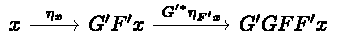
\includegraphics[width=0.95\linewidth,height=0.42\textheight,keepaspectratio]{graph-10.pdf}\end{center}
 
\begin{center}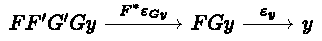
\includegraphics[width=0.95\linewidth,height=0.42\textheight,keepaspectratio]{graph-11.pdf}\end{center}
     
This composition can be shown to be associative and unital. Moreover, any equivalence $(F,G,\eta,\varepsilon):P\to Q$ admits the equivalence $(G,F,\varepsilon^{\mathrm{op}},\eta^{\mathrm{op}}):Q\to P$ as inverse (the opposite is taken pointwise).\par
 
% END S3.SS2.p4
 
% END S3.SS2
 
% BEGIN S3.SS3
 
\par\medskip\noindent\textbf{3.3 Functions induced by functors}\par
 
% BEGIN S3.SS3.p1
 
Any functor $F:P\to Q$ induces a function $\overline{F}:\overline{P}\to\overline{Q}$ between the corresponding geometric realizations defined, using the elimination principle of Proposition 3, by\par
    $\displaystyle\overline{F}x$ $\displaystyle:=\iota(Fx)$ $\displaystyle\overline{F}a$ $\displaystyle:=\gamma^{\sim}(Fa)$    
for $x:\operatorname{U}P$ and $a:x\to y$ a 1-generator in $P$, where the map $\gamma^{\sim}$ is defined in Lemma 4. The following is shown in [13, equivalence-pres].\par
 
% END S3.SS3.p1
 
% BEGIN Thmtheorem23
 
\par\medskip\noindent\textbf{Proposition 23.}\par
 
% BEGIN Thmtheorem23.p1
 
By the above construction, any functorial equivalence $(F,G,\eta,\varepsilon):P\to Q$ induces an equivalence $\|\overline{P}\|_{0}\simeq\|\overline{Q}\|_{0}$.\par
 
% END Thmtheorem23.p1
 
% END Thmtheorem23
 
% BEGIN S3.SS3.SSS0.P0.SPx1
 
\par\medskip\noindent\textbf{Proof.}\par
 
% BEGIN S3.SS3.SSS0.P0.SPx1.p1
 
Consider the functions $\|\overline{F}\|_{0}:\|\overline{P}\|_{0}\to\|\overline{Q}\|_{0}$ and $\|\overline{G}\|_{0}:\|\overline{Q}\|_{0}\to\|\overline{P}\|_{0}$. Given $x:\|\overline{P}\|_{0}$, our aim is to show that $\|\overline{G}\|_{0}\circ\|\overline{F}\|_{0}(x)=x$. Since this type is a proposition, and thus a set, it is enough to construct a function $\phi:\Pi(x:\overline{P}).(\|\overline{G}\|_{0}(|\overline{F}(x)|_{0})=x)$ which can be done by induction on $x$. Namely, for $x:\operatorname{U}P$, we have $\phi(\iota x):=|\gamma(\eta_{x}^{\mathrm{op}})|_{0}$ and, for $a:P(x,y)$, $\phi(\iota a)$ is canonically given by the fact that $\|\overline{P}\|_{0}$ is a set. We can similarly show that $\|\overline{F}\|_{0}\circ\|\overline{G}\|_{0}(y)=y$ for $y:\|\overline{Q}\|_{0}$, thus allowing us to conclude. $\hfill\blacktriangleleft$\par
 
% END S3.SS3.SSS0.P0.SPx1.p1
 
% BEGIN Thmtheorem24
 
\par\medskip\noindent\textbf{$\blacktriangleright$ Remark 24.}\par
 
% BEGIN Thmtheorem24.p1
 
It is not true that a functorial equivalence between $P$ and $Q$ induces an equivalence $\overline{P}\simeq\overline{Q}$ between the corresponding geometric realizations (as opposed to presented sets). For instance, consider the polygraph $P$ with only one 0-cell and the polygraph $Q$ with one 0-cell and one 1-cell, whose geometric realizations are respectively the point and the circle: they are functorially equivalent, but their realizations are not.\par
 
% END Thmtheorem24.p1
 
% END Thmtheorem24
 
% BEGIN S3.SS3.SSS0.P0.SPx1.p2
 
The above proposition allows us to recover in a “constructive” way the correctness property of Tietze transformations (Theorem 13). Namely, one can show [13, preservation]:\par
 
% END S3.SS3.SSS0.P0.SPx1.p2
 
% BEGIN Thmtheorem25
 
\par\medskip\noindent\textbf{Proposition 25.}\par
 
% BEGIN Thmtheorem25.p1
 
Any Tietze equivalence between two 1-polygraphs $P$ and $Q$ induces a functorial equivalence between them.\par
 
% END Thmtheorem25.p1
 
% END Thmtheorem25
 
% END S3.SS3.SSS0.P0.SPx1
 
% BEGIN S3.SS3.SSS0.P0.SPx2
 
\par\medskip\noindent\textbf{Proof.}\par
 
% BEGIN S3.SS3.SSS0.P0.SPx2.p1
 
Since functorial equivalences are closed under identities, composition and inverses, it is enough to show that any elementary Tietze transformation induces a functorial equivalence between the corresponding polygraphs.\par
  (T0)  
% BEGIN S3.I1.ix1.p1
 
Given a type $X$ and a function $\partial:X\to\operatorname{U}P$, we consider the functor $F:P\to P{\uparrow_{0}}\partial$ which is the canonical inclusion and the functor $G:P{\uparrow_{0}}\partial\to P$ defined by\par
    $\displaystyle G(x)$ $\displaystyle:=\begin{cases}x&\text{if $x:\operatorname{U}P$,}\\
\partial(x)&\text{if $x:X$,}\\
\end{cases}$ $\displaystyle G(a:x\to y)$ $\displaystyle:=\begin{cases}a::\operatorname{id}&\text{if $x,y:\operatorname{U}P$,}\\
\operatorname{id}_{x}&\text{if $x:\operatorname{U}P$ and $y:X$.}\end{cases}$    
We take $\eta_{x}:=\operatorname{id}_{x}$ for $x:\operatorname{U}P$, and $\varepsilon_{y}:F(Gy)\overset{*}{\to}y$ is defined as $\operatorname{id}_{y}$ for $y:\operatorname{U}P$ and as the 1-cell corresponding to the canonical 1-generator $\partial y\to y$ given by definition of (T0) for $y:X$.\par
 
% END S3.I1.ix1.p1
  (T1)  
% BEGIN S3.I1.ix2.p1
 
Given a function $\partial:\operatorname{S}_{0}P\to\mathcal{U}$ and functions $\partial_{x,y}:\partial(x,y)\to(x\overset{*}{\to}y)$, we consider the functor $F:P\to P{\uparrow_{1}}\partial$ which is the canonical inclusion and the functor $G$, which is the identity on 0-cells and\par
    \[G(a:x\to y):=\begin{cases}a&\text{if $a:P(x,y)$}\\
\partial_{x,y}(a)&\text{if $a:\partial(x,y)$}\end{cases}\]    
together with $\eta_{x}$ and $\varepsilon_{y}$ being both identities for $x:\operatorname{U}P$ and $y:\operatorname{U}(P{\uparrow_{1}}\partial)$.\par
 
% END S3.I1.ix2.p1
   
$\hfill\blacktriangleleft$\par
 
% END S3.SS3.SSS0.P0.SPx2.p1
 
% BEGIN S3.SS3.SSS0.P0.SPx2.p2
 
To sum up, we have introduced three notions of equivalence for 1-polygraphs: Tietze equivalence, functorial equivalence, and equivalence of presented set. The above theorems show that these three notions coincide (Theorems 13, 22, 23, and 25).\par
 
% END S3.SS3.SSS0.P0.SPx2.p2
 
% END S3.SS3.SSS0.P0.SPx2
 
% END S3.SS3
 
% END S3


% BEGIN S4
 
\par\medskip\noindent\textbf{4 Transfer of coherence}\par
 
% BEGIN S4.p1
 
In a polygraph, cells can be understood as describing the “coherence” of the data, i.e. all the relations it should satisfy. In particular, if we see a 1-polygraph as presenting a proposition (the proposition presented by the underlying 0-polygraph, in the sense of Section 1), the 1-generators should inform us that we can identify any two 0-generators, since the only relevant data is the presence of such a 0-generator. More formally, the presented set should coincide with the presented proposition: $\|\overline{P}\|_{0}=\|\overline{\operatorname{U}P}\|_{-1}$. We formalize this here and provide conditions for ensuring that we are in such a coherent situation, as well as tools to transfer coherence from a 1-polygraph to another.\par
 
% END S4.p1
 
% BEGIN S4.SS1
 
\par\medskip\noindent\textbf{4.1 Coherent presentations}\par
 
% BEGIN S4.SS1.p1
 
A coherence structure on a 1-polygraph is the data of a 1-cell $x\overset{*}{\to}y$ for every 0-sphere $x,y:\operatorname{S}_{0}P$. We say that a 1-polygraph is coherent when it admits a coherence structure. Note that any 0-polygraph $P$ can be extended into a coherent 1-polygraph by adding one 1-generator between every two 0-generators. We are however interested here in constructing coherent extensions of $P$ which are “small” (or, at least, combinatorially manageable). The techniques developed here should moreover extend to the case of higher-dimensional polygraphs, where the situation is much more involved [1].\par
 
% END S4.SS1.p1
 
% END S4.SS1
 
% BEGIN S4.SS2
 
\par\medskip\noindent\textbf{4.2 The transfer theorem}\par
 
% BEGIN S4.SS2.p1
 
Suppose given a 1-polygraph $P$, a 0-polygraph $Q^{\prime}$ and a Tietze equivalence of 0-polygraphs between $\operatorname{U}P$ and $Q^{\prime}$ (see Proposition 12). We show that when $P$ is coherent, we can transfer its coherence structure to an extension of $Q^{\prime}$, which is moreover finite when the one of $P$ is. Namely, we can construct a transferred 1-polygraph $Q$ with $\operatorname{U}Q\overset{\text{def}}{=}Q^{\prime}$ by induction on the Tietze equivalence as follows [13, extension]:\par
  (E$+$)  
% BEGIN S4.I1.ix1.p1
 
if $Q^{\prime}$ was obtained from $\operatorname{U}P$ by an elementary Tietze transformation, i.e. there is a type $X$ and a function $\partial:X\to\operatorname{U}P$ such that $Q^{\prime}=\operatorname{U}P\sqcup X$, we define\par
    \[Q(x,y):=\begin{cases}P(x,y)&\text{if $x,y:\operatorname{U}P$}\\
x=\partial(y)&\text{if $x:\operatorname{U}P$ and $y:X$}\\
\bot&\text{otherwise}\end{cases}\]    
so that there is a Tietze transformation of 1-polygraphs (T0) between $P$ and $Q$, in the sense that we have $Q:=P{\uparrow_{0}}\partial$,\par
 
% END S4.I1.ix1.p1
  (E$-$)  
% BEGIN S4.I1.ix2.p1
 
if $\operatorname{U}P$ was obtained from $Q^{\prime}$ by an elementary Tietze transformation, i.e. there is a type $X$ and a function $\partial:X\to Q^{\prime}$ such that $\operatorname{U}P=Q^{\prime}\sqcup X$, we define\par
    \[Q(x,y):=\Sigma(x^{\prime},y^{\prime}:\operatorname{U}P\sqcup X).P(x^{\prime},y^{\prime})\times(x=\partial^{\prime}(x^{\prime}))\times(y=\partial^{\prime}(y^{\prime}))\]    
where $\partial^{\prime}:Q^{\prime}\sqcup X\to Q^{\prime}$ is defined by\par
    \[\partial^{\prime}(x):=\begin{cases}x&\text{if $x:Q^{\prime}$,}\\
\partial(x)&\text{if $x:X$,}\end{cases}\]    
% END S4.I1.ix2.p1
  (E$\ast$)  
% BEGIN S4.I1.ix3.p1
 
the cases of reflexivity and transitivity are handled by identity and composition.\par
 
% END S4.I1.ix3.p1
   
% END S4.SS2.p1
 
% BEGIN Thmtheorem26
 
\par\medskip\noindent\textbf{Example 26.}\par
 
% BEGIN Thmtheorem26.p1
 
Consider the following discrete polygraphs $P$ and $Q^{\prime}$:\par
    \[P=\begin{matrix}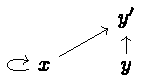
\includegraphics[width=0.24\linewidth,height=0.12\textheight,keepaspectratio]{graph-12.pdf}\end{matrix}\qquad\qquad\qquad\qquad\qquad Q^{\prime}=\begin{matrix}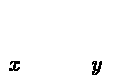
\includegraphics[width=0.24\linewidth,height=0.12\textheight,keepaspectratio]{graph-13.pdf}\end{matrix}\]    
We have that $\operatorname{U}P$ is obtained from $Q^{\prime}$ by an elementary Tietze transformation of 0-polygraphs with $X=1$ and $\partial:1\to Q^{\prime}$ defined by $\partial y^{\prime}=y$, where we write $y^{\prime}$ for the canonical element of $1$. The resulting 1-polygraph $Q$ (obtained by transfer) is thus $Q=\begin{matrix}
\includegraphics[width=0.24\linewidth,height=0.12\textheight,keepaspectratio]{graph-14.pdf}\end{matrix}$. The polygraphs $P$ and $Q$ are Tietze equivalent: we have the Tietze transformations\par
    
\begin{center}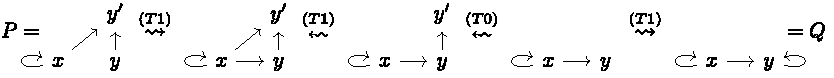
\includegraphics[width=0.95\linewidth,height=0.42\textheight,keepaspectratio]{graph-15.pdf}\end{center}
    
We will show in Theorem 28 that there is always a Tietze equivalence when $P$ is coherent, but the equivalence produced by the proof of the theorem will rather be the following one:\par
    
\begin{center}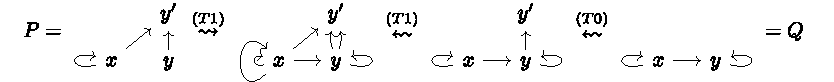
\includegraphics[width=0.95\linewidth,height=0.42\textheight,keepaspectratio]{graph-16.pdf}\end{center}
    
% END Thmtheorem26.p1
 
% END Thmtheorem26
 
% BEGIN Thmtheorem27
 
\par\medskip\noindent\textbf{$\blacktriangleright$ Remark 27.}\par
 
% BEGIN Thmtheorem27.p1
 
Consider the variant of the previous example where $P$ is the same 1-polygraph with the 1-generator $y\to y^{\prime}$ removed and $Q^{\prime}$ is left unchanged. In this case, the resulting polygraph $Q$ is the same as in previous example. However, the two polygraphs are not Tietze equivalent. Namely, we have $\|\overline{P}\|_{0}=2$ and $\|\overline{Q}\|_{0}=1$, and a Tietze equivalence would thus be in contradiction with Theorem 13. Note that the polygraph $P$ is not coherent.\par
 
% END Thmtheorem27.p1
 
% END Thmtheorem27
 
% BEGIN S4.SS2.p2
 
We now show the following transfer theorem which states that a Tietze equivalence between 0-polygraphs can be extended as a Tietze equivalence between 1-polygraphs when one of them is coherent [13, transfer]. Remark 27 illustrates why the coherence hypothesis is required.\par
 
% END S4.SS2.p2

% BEGIN Thmtheorem28
 
\par\medskip\noindent\textbf{Theorem 28 (Transfer theorem).}\par
 
% BEGIN Thmtheorem28.p1
 
When $P$ is coherent, the above polygraphs $P$ and $Q$ are Tietze equivalent.\par
 
% END Thmtheorem28.p1
 
% END Thmtheorem28

% BEGIN S4.SS2.SSS0.P0.SPx1
 
\par\medskip\noindent\textbf{Proof.}\par
 
% BEGIN S4.SS2.SSS0.P0.SPx1.p1
 
As above for the construction of $Q$, we reason by induction on the Tietze equivalence between $\operatorname{U}P$ and $Q^{\prime}$. In the case (E$+$), $Q$ is obtained from $P$ by a Tietze transformation (T0) and we conclude immediately.\par
 
% END S4.SS2.SSS0.P0.SPx1.p1
 
% BEGIN S4.SS2.SSS0.P0.SPx1.p2
 
The interesting case to handle is (E$-$), where $\operatorname{U}P=Q^{\prime}\sqcup X$ for some type $X$ and $\partial:X\to Q^{\prime}$. In this case, we are going to construct a series of 1-polygraphs, which are elementarily Tietze equivalent, thus exhibiting a Tietze equivalence between $P$ and $Q$, as illustrated in Example 26. It is natural to consider the 1-polygraph $R$ obtained from $Q$ by performing the “same Tietze transformation”, but with 1-polygraphs instead of 0-polygraphs, i.e. to consider $R:=Q{\uparrow_{0}}\partial$. Clearly, $P$ and $R$ have the same 0-generators, but not the same 1-generators, and we will show that both are equivalent to a third 1-polygraph $S$, still with the same 0-cells, and with the union of the 1-generators of $P$ and those of $Q$ as 1-cells. Formally, we thus define the polygraph $S$, as well as a variant $\tilde{S}$, by\par
    $\displaystyle\operatorname{U}S$ $\displaystyle=\operatorname{U}\tilde{S}=\operatorname{U}P$ $\displaystyle S(x,y)$ $\displaystyle=P(x,y)\sqcup Q(x,y)$ $\displaystyle\tilde{S}(x,y)$ $\displaystyle=Q(x,y)\sqcup P(x,y)$    
We claim that we have a series of Tietze transformations\par
    \[P\quad\overset{(T1)}{\rightsquigarrow}\quad S\quad\simeq\quad\tilde{S}\quad\overset{(T1)}{\mathrel{\rotatebox[origin={c}]{180.0}{$\rightsquigarrow$}}}\quad R\quad\overset{(T0)}{\mathrel{\rotatebox[origin={c}]{180.0}{$\rightsquigarrow$}}}\quad Q\]    
as illustrated in Example 26. Those can be constructed as follows.\par
  
\par\noindent  $\blacksquare$ 
% BEGIN S4.I2.i1.p1
 
$P\overset{(T1)}{\rightsquigarrow}S$. The coherence of $P$ provides us, for every 0-sphere $(x,y)$, with a cell $x\overset{*}{\to}y$. This allows us to define a family of functions, indexed by 0-spheres $(x,y):\operatorname{S}_{0}P$, $\partial_{x,y}:S(x,y)\to(x\overset{*}{\to}y)$, so that we have $S\overset{\text{def}}{=}P{\uparrow_{1}}\partial$.\par
 
% END S4.I2.i1.p1
 
 
\par\noindent  $\blacksquare$ 
% BEGIN S4.I2.i2.p1
 
$S\simeq\tilde{S}$. The polygraphs $S$ and $\tilde{S}$ are clearly isomorphic, in the sense of Section 3.1.\par
 
% END S4.I2.i2.p1
 
 
\par\noindent  $\blacksquare$ 
% BEGIN S4.I2.i3.p1
 
$R\overset{(T1)}{\rightsquigarrow}\tilde{S}$. We define a family of functions indexed by 0-spheres $(x,y):\operatorname{S}_{0}R$, and $\tilde{\partial}_{x,y}:P(x,y)\to(x\overset{*}{\to}y)$ by\par
    \[\tilde{\partial}_{x,y}(a):=\left\{\begin{array}[]{l@{\quad}l@{\qquad}l@{\quad}l}a::\operatorname{id}&\text{if $x:Q^{\prime}$ and $y:Q^{\prime}$}&\tau_{x}::^{\prime}a::\operatorname{id}&\text{if $x:X$ and $y:Q^{\prime}$}\\
a::\tau_{y}::\operatorname{id}&\text{if $x:Q^{\prime}$ and $y:X$}&\tau_{x}::^{\prime}a::\tau_{y}::\operatorname{id}&\text{if $x:X$ and $y:X$}\end{array}\right.\]    
where, for $x:X$, the 1-generator $\tau_{x}:\partial x\to x$ is canonically given by the definition of $R$ from $Q$ by a Tietze transformation (T0). We then have $\tilde{S}\overset{\text{def}}{=}R{\uparrow_{1}}\tilde{\partial}$.\par
 
% END S4.I2.i3.p1
 
 
\par\noindent  $\blacksquare$ 
% BEGIN S4.I2.i4.p1
 
$R\overset{(T0)}{\rightsquigarrow}Q$. The transformation (T0) from $Q$ to $R$ is given by the very definition of $R$.\par
 
% END S4.I2.i4.p1
 
  
$\hfill\blacktriangleleft$\par
 
% END S4.SS2.SSS0.P0.SPx1.p2
 
% END S4.SS2.SSS0.P0.SPx1
 
% END S4.SS2
 
% END S4

\begin{thebibliography}{99}

% BEGIN bib
 
\par\medskip\noindent\textbf{References}\par
  
\par\noindent  [1]  Dimitri Ara, Albert Burroni, Yves Guiraud, Philippe Malbos, François Métayer, and Samuel Mimram.  Polygraphs: from rewriting to higher categories.  Cambridge University Press, 2025.  
 
\par\noindent  [2]  Franz Baader and Tobias Nipkow.  Term rewriting and all that.  Cambridge University Press, 1998.  
 
\par\noindent  [3]  Christopher J Dean, Eric Finster, Ioannis Markakis, David Reutter, and Jamie Vicary.  Computads for weak $\omega$-categories as an inductive type.  Advances in Mathematics, 450, 2024.  
 
\par\noindent  [4]  Yves Guiraud and Philippe Malbos.  Identities among relations for higher-dimensional rewriting systems.  In Operads 2009, volume 26 of Séminaires et congrès, pages 145–161. Société Mathématique de France, 2013.  
 
\par\noindent  [5]  Yves Guiraud and Philippe Malbos.  Polygraphs of finite derivation type.  Mathematical Structures in Computer Science, 28(2):155–201, 2018.  doi:10.1017/S0960129516000220.  
 
\par\noindent  [6]  Allen Hatcher.  Algebraic Topology.  Cambridge University Press, 2002.  
 
\par\noindent  [7]  Simon Henry and Samuel Mimram.  Tietze equivalences as weak equivalences.  Applied Categorical Structures, 30(3):453–483, 2022.  doi:10.1007/S10485-021-09662-W.  
 
\par\noindent  [8]  Donald E. Knuth and Peter B. Bendix.  Simple word problems in universal algebras.  In Computational problems in abstract algebra, pages 263–297. Pergamon, 1970.  
 
\par\noindent  [9]  Nicolai Kraus and Jakob von Raumer.  Path spaces of higher inductive types in homotopy type theory.  In 2019 34th Annual ACM/IEEE Symposium on Logic in Computer Science (LICS), pages 1–13. IEEE, 2019.  doi:10.1109/LICS.2019.8785661.  
 
\par\noindent  [10]  Nicolai Kraus and Jakob von Raumer.  A rewriting coherence theorem with applications in homotopy type theory.  Mathematical Structures in Computer Science, 32(7):982–1014, 2022.  doi:10.1017/S0960129523000026.  
 
\par\noindent  [11]  Yves Lafont.  A new finiteness condition for monoids presented by complete rewriting systems (after Craig C. Squier).  Journal of Pure and Applied Algebra, 98(3):229–244, 1995.  
 
\par\noindent  [12]  Yves Lafont, François Métayer, and Krzysztof Worytkiewicz.  A folk model structure on omega-cat.  Advances in Mathematics, 224(3):1183–1231, 2010.  
 
\par\noindent  [13]  Samuel Mimram.  Polygraphs in Agda.  Software, swhId: swh:1:dir:27f2a0c3a496b72c3f4cd458ab51ea174f448eb7 (visited on 2025-06-23).  URL: https://github.com/smimram/agda-polygraphs, doi:10.4230/artifacts.23666.  
 
\par\noindent  [14]  Samuel Mimram.  Categorical coherence from term rewriting systems.  In Marco Gaboardi and Femke van Raamsdonk, editors, 8th International Conference on Formal Structures for Computation and Deduction (FSCD), volume 260 of LIPIcs, pages 16:1–16:17. Schloss Dagstuhl, 2023.  doi:10.4230/LIPICS.FSCD.2023.16.  
 
\par\noindent  [15]  Maxwell Herman Alexander Newman.  On theories with a combinatorial definition of “equivalence”.  Annals of mathematics, 43(2):223–243, 1942.  
 
\par\noindent  [16]  Kristina Sojakova, Floris van Doorn, and Egbert Rijke.  Sequential colimits in homotopy type theory.  In Holger Hermanns, Lijun Zhang, Naoki Kobayashi, and Dale Miller, editors, LICS ’20: 35th Annual ACM/IEEE Symposium on Logic in Computer Science, pages 845–858. ACM, 2020.  doi:10.1145/3373718.3394801.  
 
\par\noindent  [17]  Craig C Squier, Friedrich Otto, and Yuji Kobayashi.  A finiteness condition for rewriting systems.  Theoretical Computer Science, 131(2):271–294, 1994.  doi:10.1016/0304-3975(94)90175-9.  
 
\par\noindent  [18]  Heinrich Tietze.  Über die topologischen Invarianten mehrdimensionaler Mannigfaltigkeiten.  Monatshefte für Mathematik und Physik, 19:1–118, 1908.  
 
\par\noindent  [19]  The Univalent Foundations Program.  Homotopy Type Theory: Univalent Foundations of Mathematics.  https://homotopytypetheory.org/book, Institute for Advanced Study, 2013.  
 
\par\noindent  [20]  Andrea Vezzosi, Anders Mörtberg, and Andreas Abel.  Cubical Agda: a dependently typed programming language with univalence and higher inductive types.  Proceedings of the ACM on Programming Languages, 3:1–29, 2019.  doi:10.1145/3341691.  
  
% END bib
\end{thebibliography}
\end{document}
